\documentclass[a4paper, 11pt]{article}
\usepackage{amsmath}
\usepackage{graphicx}

\title{ASSIGNMENT 4 \\ The Photoelectric Equation of Einstein}
\author{Siddhartha R CH22B021}
\date{}

\begin{document}

\maketitle

\section{Introduction}

The photoelectric effect is a phenomenon in which electrons are emitted from a material surface when exposed to light of sufficient energy. It was first discovered by Heinrich Hertz in 1887 and later explained by Albert Einstein in 1905. The photoelectric effect played a crucial role in the development of quantum mechanics and helped establish the wave-particle duality of light. The photoelectric equation, formulated by Einstein, describes the relationship between the energy of incident photons, the work function of a material, and the kinetic energy of emitted electrons.

\section{The Photoelectric Equation}

The photoelectric equation is given by:

\begin{equation}
    E = h\nu - \phi
\end{equation}

where $E$ is the energy of the emitted electron, $h$ is Planck's constant ($6.62607015 \times 10^{-34}\, \text{J}\cdot \text{s}$), $\nu$ is the frequency of the incident light, and $\phi$ is the work function of the material. The work function represents the minimum amount of energy required to remove an electron from the material surface.

The equation shows that the energy of the emitted electron ($E$) is equal to the energy of the incident photon ($h\nu$) minus the work function ($\phi$). If the incident photon's energy is insufficient to overcome the work function, no electrons will be emitted. This implies that even if the intensity of the incident light is increased, no electrons will be emitted unless the individual photons have sufficient energy.


\section{Explanation and Implications}


If the energy of the incident photon is greater than the work function, the excess energy is converted into the kinetic energy of the emitted electron. However, if the energy of the photon is less than the work function, the electron cannot be emitted, regardless of the light intensity. 

The photoelectric equation demonstrates the particle-like behavior of light, where photons transfer discrete amounts of energy. It also explains the observed phenomenon that increasing the intensity of incident light increases the number of emitted electrons, but not their kinetic energy. The intensity affects only the number of photons, not their individual energies.

Moreover, the equation supports the concept of wave-particle duality by relating the energy of photons (wave property) to the kinetic energy of electrons (particle property). The photoelectric effect cannot be explained solely by classical wave theory, highlighting the need for quantum mechanics to understand the behavior of light and matter at the atomic scale.
\begin{figure}[h]
    \centering
    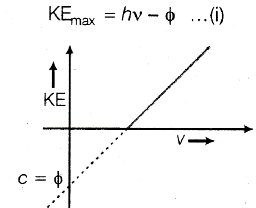
\includegraphics[width=0.8\textwidth]{IMG PHOTOELECTRIC.png}
    \caption{Illustration of the photoelectric effect}
    \label{fig:photoelectric}
\end{figure}


\section{Conclusion}

In conclusion, the photoelectric equation proposed by Einstein provides a fundamental understanding of the photoelectric effect. It establishes the relationship between the energy of incident photons, the work function of a material, and the kinetic energy of emitted electrons. This equation played a significant role in the development of quantum mechanics, confirming the wave-particle duality of light and advancing our understanding.
\footnote{I took this equation from NCERT CLASS 12 textbook}

\end{document}
